\textit{Response.}

\begin{enumerate}[a)]
	\item We begin be deriving a formula analogous to It\^{o}'s formula for Eqn.~\ref{eqn:model_6}. In particular, for an SDE of the form

	\begin{equation}
		dx = \func{a}{t,\ x}\,dt + \func{b}{t,\ x}\,dW + \func{\sigma}{t,\ x}\,dW_A,
	\end{equation}		
	
	we have the Taylor's series expansion
	
	\begin{align}
		d\func{f}{t,\ x} &= \pdv{f}{t}\,dt + \pdv{f}{x}\,dx + \frac{1}{2}\,\gpr{\pdv[2]{f}{t}\,\gpr{dt}^2 + 2\,\pdv[2]{f}{t}{x}\,\gpr{dt}\,\gpr{dx} + \pdv[2]{f}{x}\,\gpr{dx}^2} + \dots \nonumber \\
			&= \pdv{f}{t}\,dt + \pdv{f}{x}\,\gpr{\func{a}{t,\ x}\,dt + \func{b}{t,\ x}\,dW + \func{\sigma}{t,\ x}\,dW_A} \nonumber \\
				&\qquad + \frac{1}{2}\,\pdv[2]{f}{t}\,\gpr{dt}^2 \nonumber \\
				&\qquad + \pdv[2]{f}{t}{x}\,\gpr{dt}\,\gpr{\func{a}{t,\ x}\,dt + \func{b}{t,\ x}\,dW + \func{\sigma}{t,\ x}\,dW_A} \nonumber \\
				&\qquad + \frac{1}{2}\,\pdv[2]{f}{x}\,\gpr{\func{a}{t,\ x}\,dt + \func{b}{t,\ x}\,dW + \func{\sigma}{t,\ x}\,dW_A}^2.
	\end{align}
	
	Note that the noise terms $\gpr{dW}^2$ and $\gpr{d{W_{A}}}^2$ are of order $\ord{dt}$, and that we may substitute them for $dt$ by the variance of the Weiner process. Further, the terms $\gpr{dt}^2$, $dt\,dW$, and $dt\,d{W_A}$ all tend to zero faster than $dt$. Hence, taking this equation in the limit as $dt$ tend to zero and replacing $\gpr{dW}^2$ and $\gpr{d{W_{A}}}^2$ by $dt$ and replacing $\gpr{dt}^2$, $dt\,dW$, and $dt\,d{W_A}$ by zero, we may group the terms of this equation together into $dt$, $dW$, $dW_{A}$, and $dW\,dW_{A}$ terms
	
	\begin{align}
		d\func{f}{t,\ x} &= \gpr{\pdv{f}{t} + \func{a}{t,\ x}\,\pdv{f}{x} + \frac{1}{2}\,\gpr{\gpr{\func{b}{t,\ x}}^2 + \gpr{\func{\sigma}{t,\ x}}^2}\,\pdv[2]{f}{x}}\,dt \nonumber \\
				&\qquad + \func{b}{t,\ x}\,\pdv{f}{x}\,dW + \func{\sigma}{t,\ x}\,\pdv{f}{x}\,dW_A \nonumber \\
				&\qquad + \frac{1}{2}\,\func{b}{t,\ x}\,\func{\sigma}{t,\ x}\,\pdv[2]{f}{x}\,\gpr{dW}\,\gpr{dW_{A}}. \label{eqn:model_6_ito}
	\end{align}
	
	Now, to find the evolution of the mean of $x$, we may simply take the ensemble average of Eqn.~\ref{eqn:model_6}
	
	\begin{equation}
		\gang{dx} = d\gang{x} = \gpr{F + a\,\gang{x} + b\,\gang{x^2} - c\,\gang{x^3}}\,dt.
	\end{equation}
	
	The evolution of the variance of $x$ is given by 
	
	\begin{equation}
		d\vr{x} = d\gbkt{\gang{x^2} - \gang{x}^2} = d\gang{x^2} - 2\,\gang{x}\,d\gang{x}.
		\label{eqn:model_6_var}
	\end{equation}
	
	We may obtain $d\gang{x^2}$ using Eqn.~\ref{eqn:model_6_ito}
	
	\begin{align}
		d \gang{x^2} &= \gang{d \gbkt{x^2}} = \gang{\gpr{0 + \gpr{F + a\,x + b\,x^2 - c\,x^3}\,\gpr{2\,x} + \frac{1}{2}\,\gpr{\gpr{A - B\,x}^2 + \sigma^2}\,\gpr{2}}}\,dt \nonumber \\
				&= \gang{\gpr{2\,x\,\gpr{F + a\,x + b\,x^2 - c\,x^3} + \gpr{A - B\,x}^2 + \sigma^2}}\,dt \nonumber \\
				&= \gpr{\gpr{A^2 + \sigma^2} + \gpr{2\,F - 2\,A\,B}\,\gang{x} + \gpr{2\,a + B^2}\,\gang{x^2} + \gpr{2\,b}\,\gang{x^3} + \gpr{-2\,c}\,\gang{x^4}}\,dt.
	\end{align}
	
	The second term of Eqn.~\ref{eqn:model_6_var} is given by
	
	\begin{equation}
		2\,\gang{x}\,d\gang{x} = \gpr{2\,F\,\gang{x} + 2\,a\,\gpr{\gang{x}}^2 + 2\,b\,\gang{x}\,\gang{x^2} - 2\,c\,\gang{x}\,\gang{x^3}}\,dt.
	\end{equation}
	
	Therefore, we have
	
	\begin{align}
		d\vr{x} &= \left(\gpr{A^2 + \sigma^2} + \gpr{-2\,A\,B}\,\gang{x} + 2\,a\,\vr{x} + B^2\,\gang{x^2} \right. \nonumber \\
				&\qquad \left. + 2\,b\,\gpr{\gang{x^3} - \gang{x}\,\gang{x^2}} - 2\,c\,\gpr{\gang{x^4} - \gang{x}\,\gang{x^3}} \right)\,dt
	\end{align}
	
	We may simplify these equations for the evolution of $\gang{x}$ and $\vr{x}$ using the quasi-Gaussian closure. In particular, we have that the third-order central moment is zero
	
	\begin{equation}
		\gang{\gpr{x - \gang{x}}^3} = \gang{x^3} - 3\,\gang{x}\,\gang{x^2} + 2\,\gang{x}^3 = 0
	\end{equation}
	
	and that the fourth-order central moment is of the same form as a typical Gaussian distribution
	
	\begin{equation}
		\gang{\gpr{x - \gang{x}}^4} = \gang{x^4} - 4\,\gang{x}\,\gang{x^3} + 6\,\gang{x}^2\,\gang{x^2} - 3\,\gang{x}^4 = 3\,\gpr{\vr{x}}^2.
	\end{equation}
	
	Using this, we may write equations for the first four non-central moments
	
	\begin{subequations}
		\begin{align}
			\gang{x} &= \gang{x}, \\
			\gang{x^2} &= \vr{x} + \gang{x}^2, \\
			\gang{x^3} &= 3\,\gang{x}\,\gang{x^2} - 2\,\gang{x}^3 = 3\,\gang{x}\,\vr{x} + \gang{x}^3, \\
			\gang{x^4} &= 3\,\gpr{\vr{x}}^2 + 6\,\gang{x}^2\,\vr{x} + \gang{x}^4.
		\end{align}
	\end{subequations}
	
	Hence, we may write the equations for the evolution of the mean and the variance
	
	\begin{subequations}
		\begin{align}
			d\gang{x} &= \gpr{F + a\,\gang{x} + b\,\gpr{\vr{x} + \gang{x}^2} - c\,\gpr{3\,\gang{x}\,\vr{x} + \gang{x}^3}}\,dt \nonumber \\
				&= \gpr{F + \gpr{a\,\gang{x} + b\,\gang{x}^2 - c\,\gang{x}^3} + \gpr{b - 3\,c\,\gang{x}}\,\vr{x}}\,dt
		\end{align}
		\begin{align}
			d\vr{x} &= \left(\gpr{A^2 + \sigma^2} + \gpr{-2\,A\,B}\,\gang{x} + 2\,a\,\vr{x} + B^2\,\gpr{\vr{x} + \gang{x}^2} \right. \nonumber \\
					&\qquad \left. + 2\,b\,\gpr{\gpr{3\,\gang{x}\,\vr{x} + \gang{x}^3} - \gang{x}\,\gpr{\vr{x} + \gang{x}^2}} \right. \nonumber \\
					&\qquad \left. - 2\,c\,\gpr{\gpr{3\,\gpr{\vr{x}}^2 + 6\,\gang{x}^2\,\vr{x} + \gang{x}^4} - \gang{x}\,\gpr{3\,\gang{x}\,\vr{x} + \gang{x}^3}} \right)\,dt \nonumber \\
				&= \left(\gpr{A^2 + \sigma^2} + \gpr{-2\,A\,B\,\gang{x} + B^2\,\gang{x}^2}  \right. \nonumber \\
					&\qquad \left. + \gpr{2\,a + B^2 + 4\,b\,\gang{x} - 6\,c\,\gang{x}^2}\,\vr{x} - 6\,c\,\gpr{\vr{x}}^2 \right)\,dt.
		\end{align}
	\end{subequations}
	
	\item The Fokker-Planck equation associated with Eqn.~\ref{eqn:model_6} is given by
	
	\begin{equation}
		\pdv{p}{t} = -\pdv{x}\gbkt{\gpr{F + a\,x + b\,x^2 - c\,x^3}\,p} + \frac{1}{2}\,\pdv[2]{x}\gbkt{\gpr{\gpr{A - B\,x}^2 + \sigma^2}\,p}.
	\end{equation}
	
	The simplest equilibrium distribution is when $A = B = 0$, which is
	
	\begin{equation}
		\func{p_{eq}}{x} = \mathcal{C}\,e^{\frac{2}{\sigma^2}\,\gpr{F\,x + \frac{a}{2}\,x^2 + \frac{b}{3}\,x^3 - \frac{c}{4}\,x^4}}
	\end{equation}
	
	where $\mathcal{C}$ is a normalization constant to ensure $\int_{\mathbb{R}} \func{p_{eq}}{x}\,dx = 1$.
	
	To obtain the bimodal distribution and example trajectory shown in Figures~\ref{fig:6b_pdf} and \ref{fig:6b_traj}, respectively, we used the following parameter values
	
	\begin{equation}
		\sigma = 1,\qquad F = 0,\qquad a = 3,\qquad b = 0,\qquad c = 3.
	\end{equation}
	
	\begin{figure}[H]
		\centering
		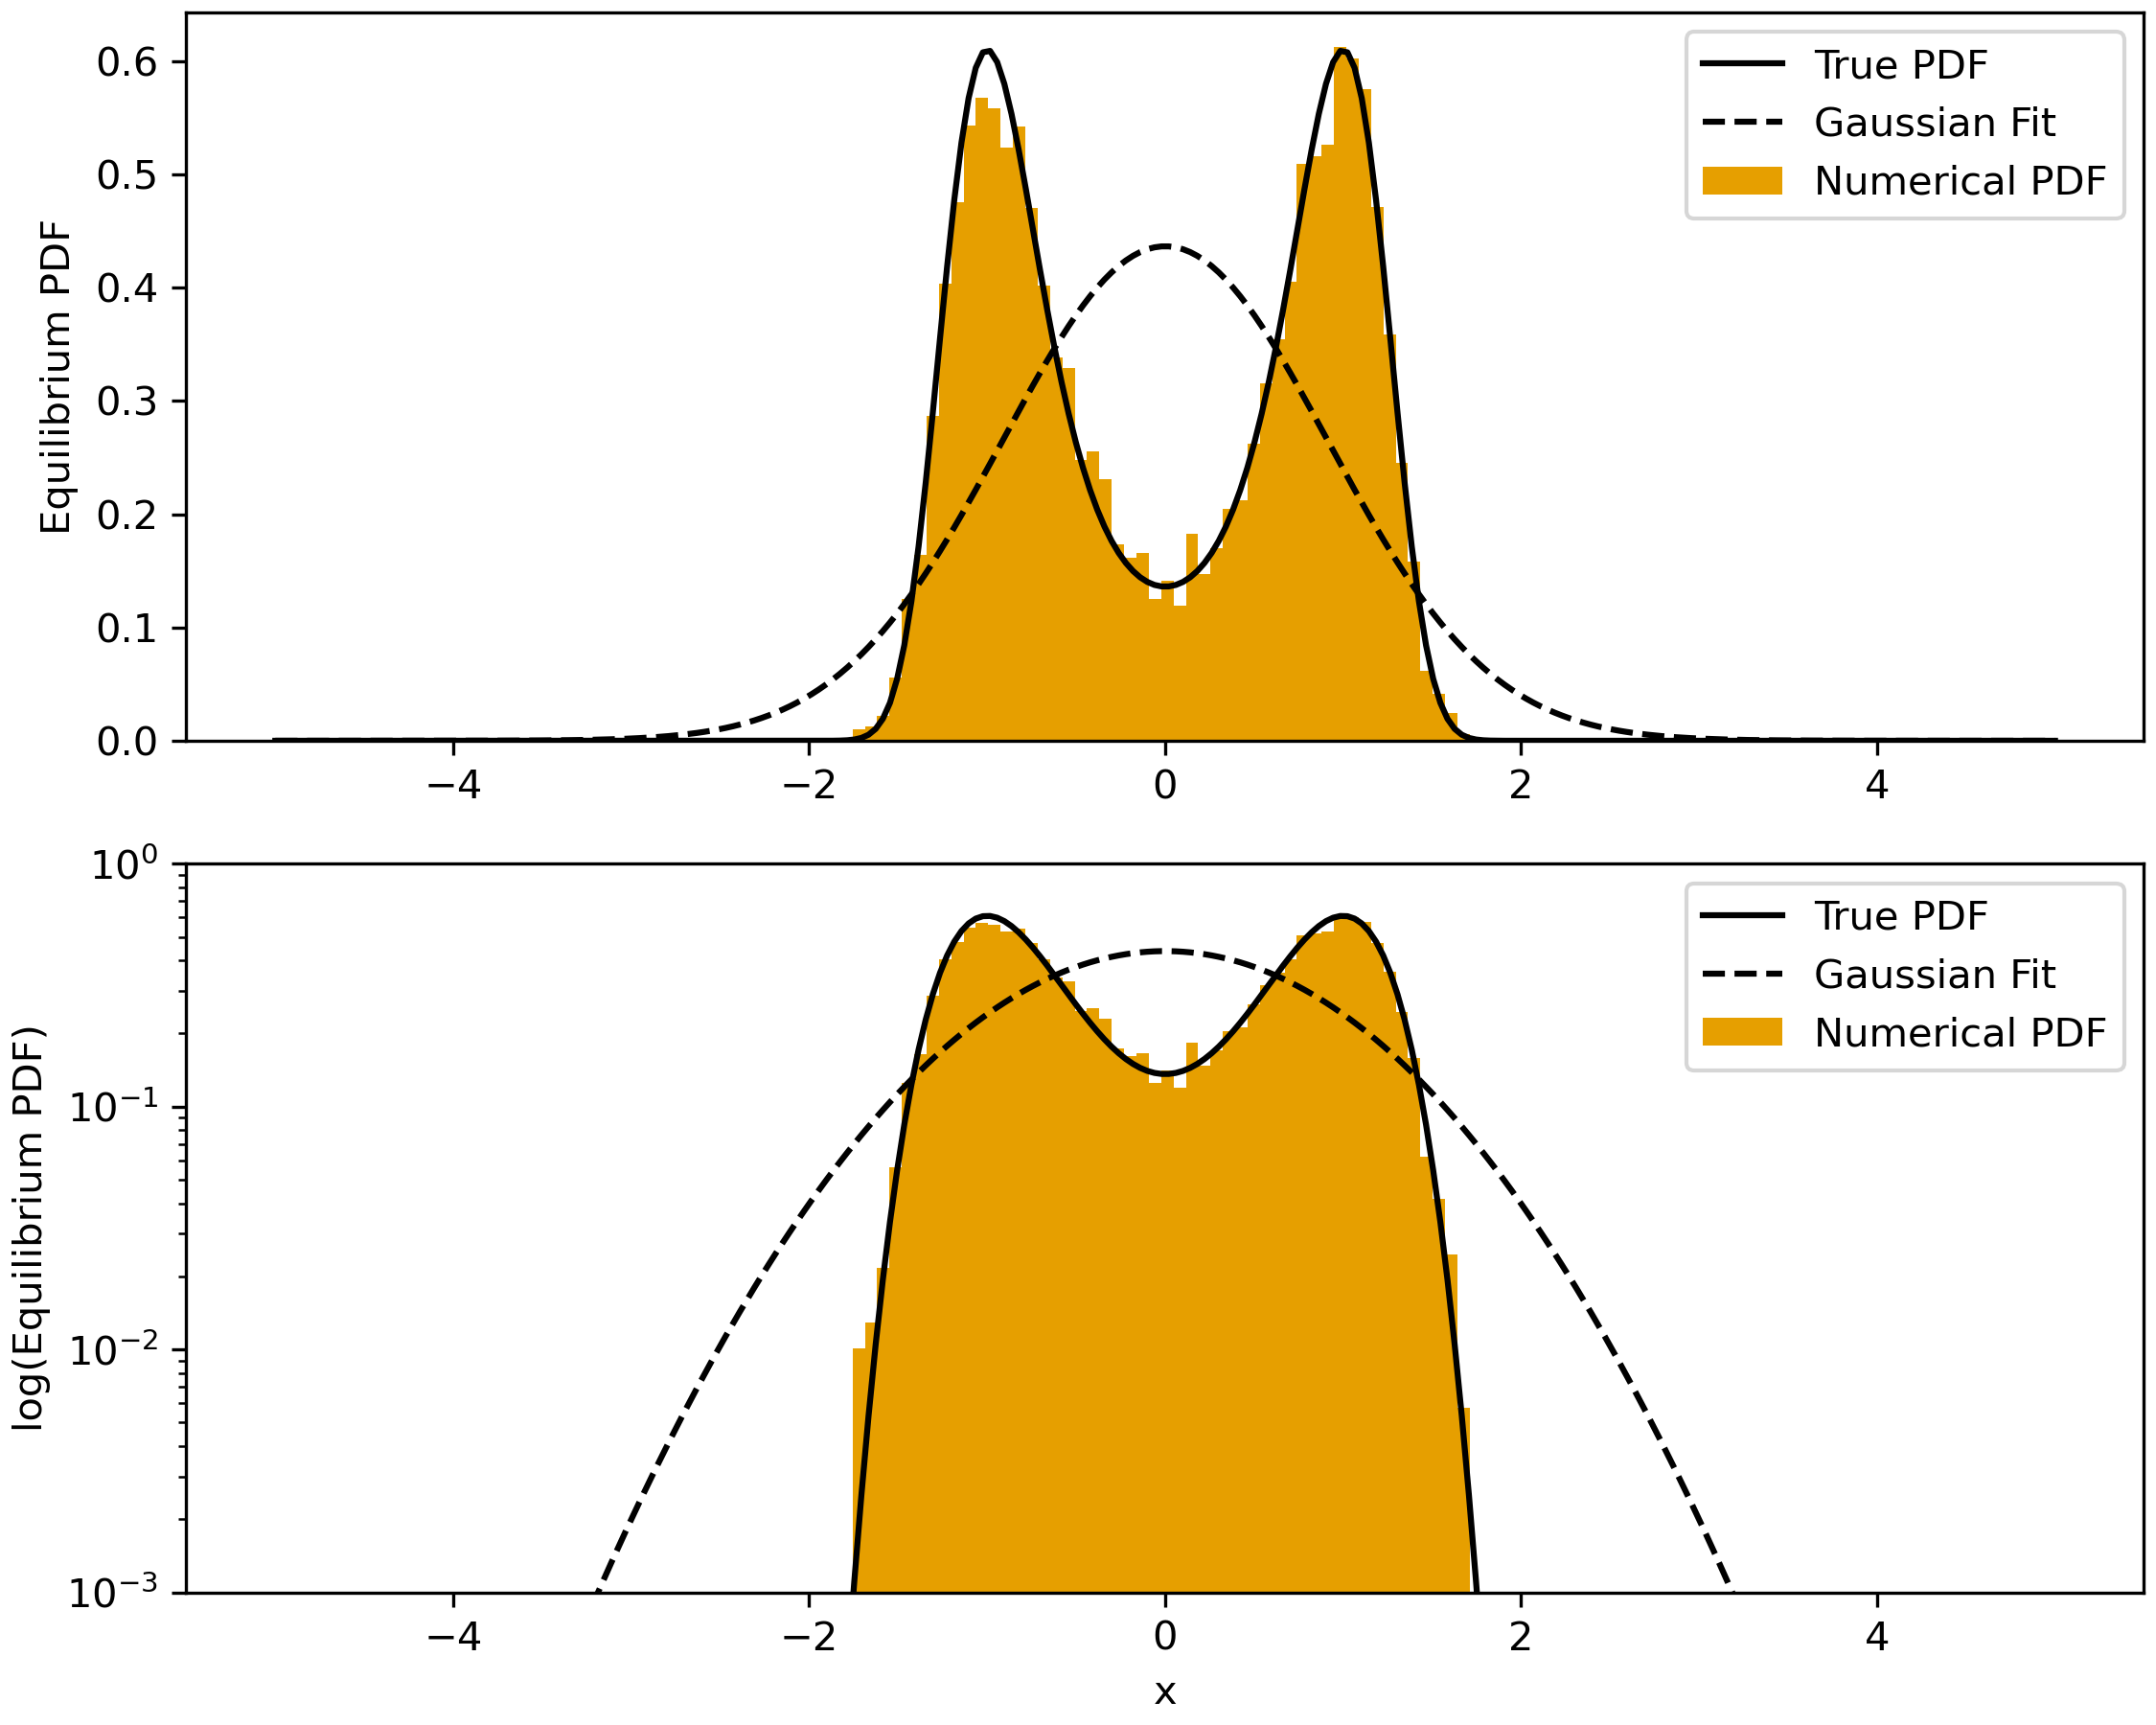
\includegraphics[width=0.75\textwidth]{../../src/6b_pdf.png}
		\caption{The equilibrium probability density function for Eqn.~\ref{eqn:model_6} (solid) along with a Gaussian fit (dashed) and a histogram generated from the 1000\textsuperscript{th} time-step ($dt = 0.01$) of 10000 trials (orange), with parameters $\sigma = 1$, $F = 0$, $a = 3$, $b = 0$, and $c = 3$, each initialized as $x = 0$.}
		\label{fig:6b_pdf}
	\end{figure}
	
	\begin{figure}[H]
		\centering
		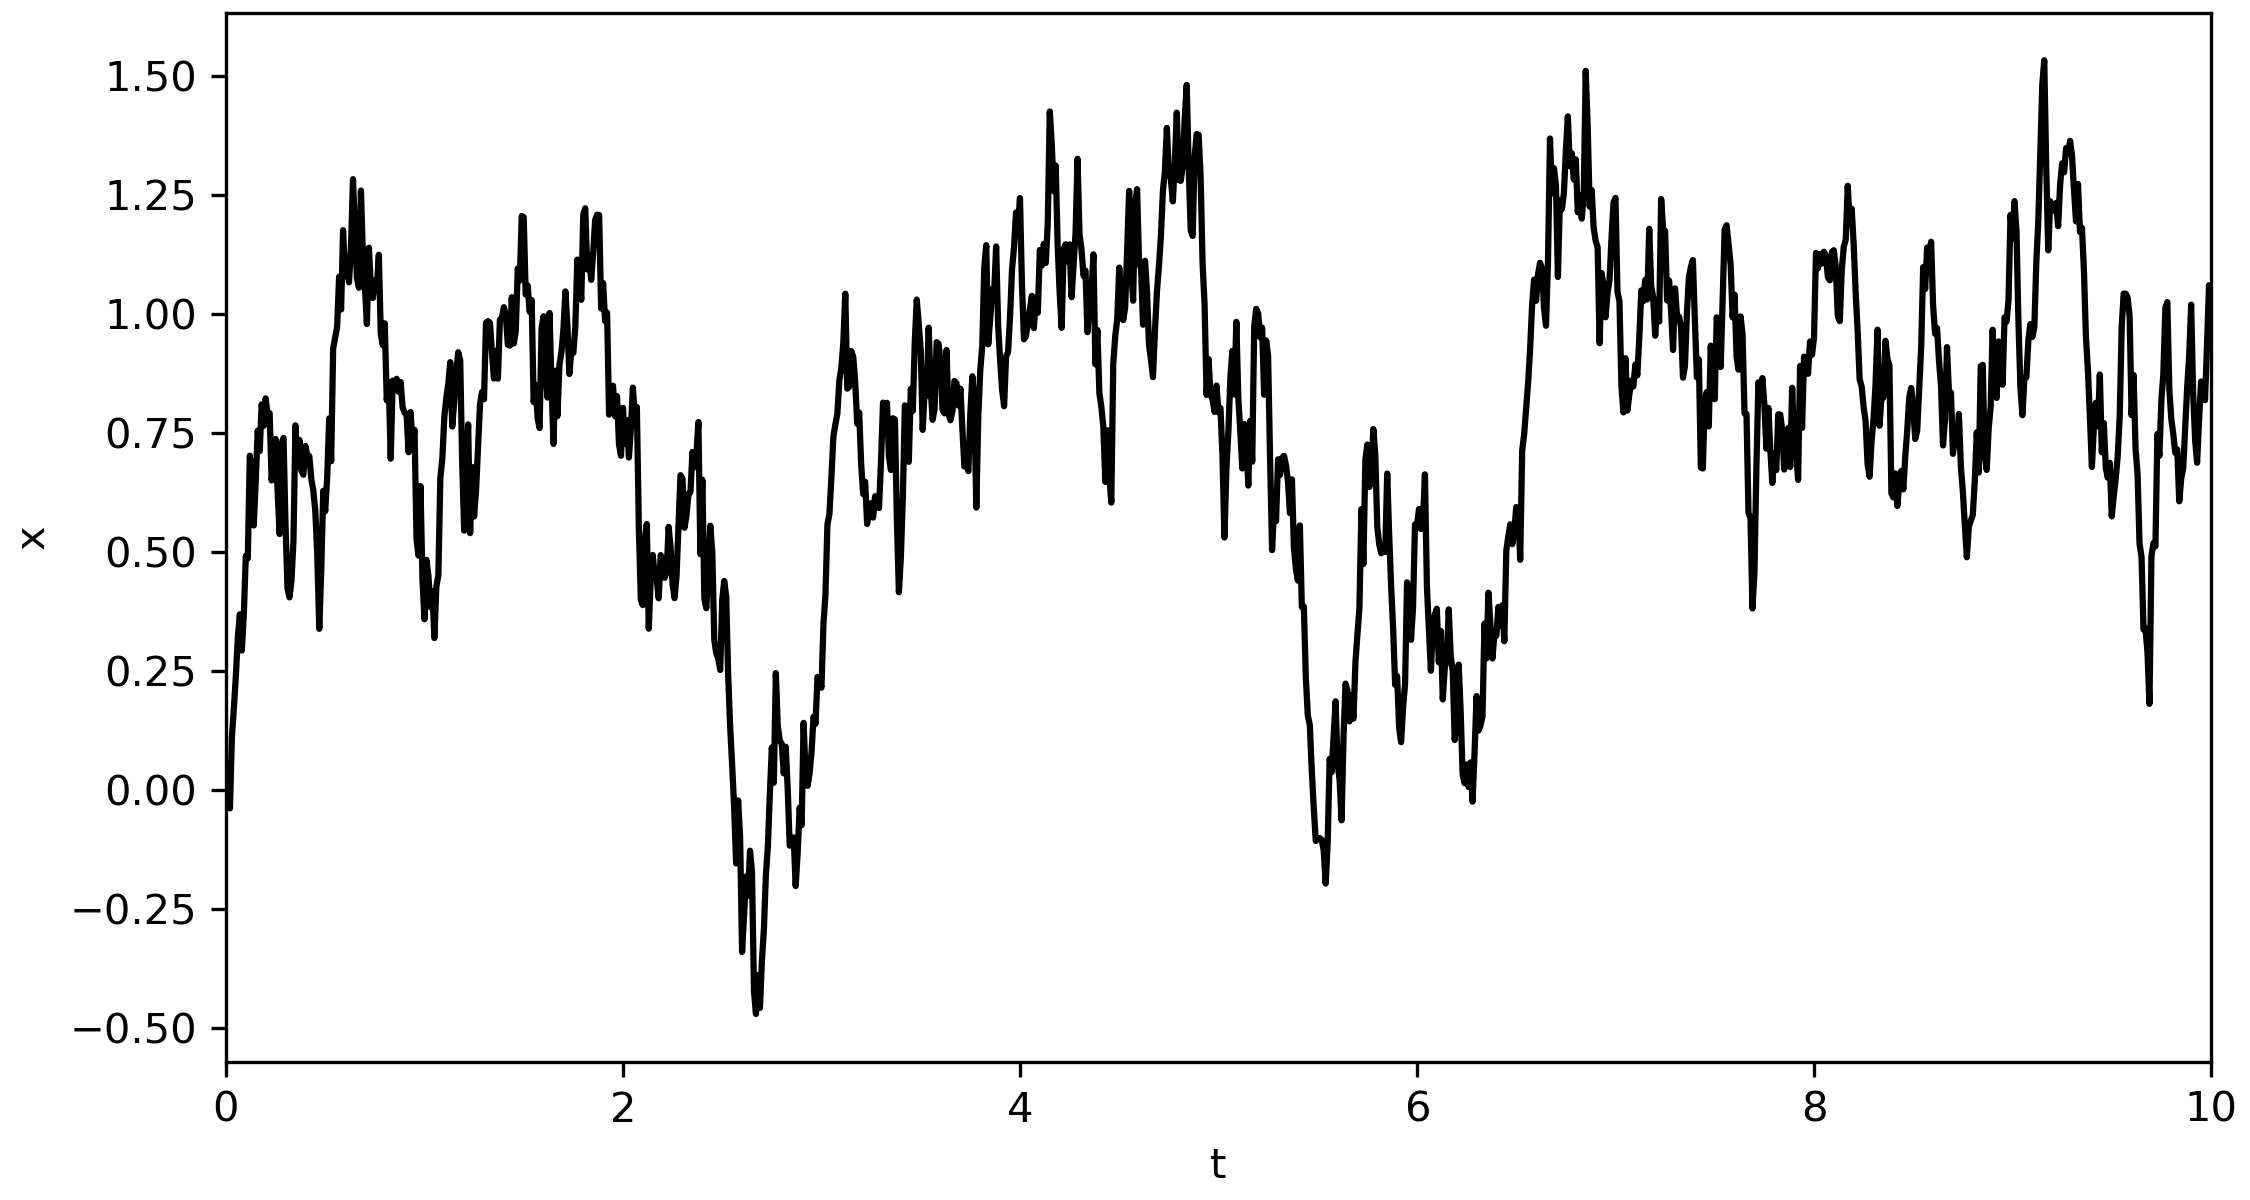
\includegraphics[width=0.75\textwidth]{../../src/6b_traj.png}
		\caption{An example trajectory for Eqn.~\ref{eqn:model_6} for 1000 time-steps of size $dt = 0.01$ with parameters $\sigma = 1$, $F = 0$, $a = 3$, $b = 0$, and $c = 3$, initialized as $x = 0$.}
		\label{fig:6b_traj}
	\end{figure}
	
	Source code is available from the GitHub repository
	
	\begin{center}
		\url{https://github.com/jasonltorchinsky/MATH833_HW/releases/tag/midterm}
	\end{center}

	and is given in Appendix~\ref{app:code_6b}. In short, the code takes a input parameters \texttt{-s}, \texttt{-F}, \texttt{-a}, \texttt{-b}, and \texttt{-c} which correspond to $\sigma$, $F$, $a$, $b$, and $c$, respectively, assuming $A = B = 0$. The code then calculates the equilibrium distribution and a Gaussian approximation using the mean and variance of this equilibrium distribution. It then simulates 10000 trials for 1000 time-steps, and plots the normalized histogram as well. Finally, it simulates and plots a single trajectory for 1000 time-steps.

	\item Using the same parameters as in part b), with slight modifications to the code which is available from the GitHub repository
	
	\begin{center}
		\url{https://github.com/jasonltorchinsky/MATH833_HW/releases/tag/midterm}
	\end{center}

	and is given in Appendix~\ref{app:code_6c}, we may see that the mean and variance quickly decay from their initial values towards one and zero, respectively, and then slowly tend toward the mean and variance of the equilibrium distribution, shown in Figure~\ref{fig:6c_evo}.
	
	\begin{figure}[H]
		\centering
		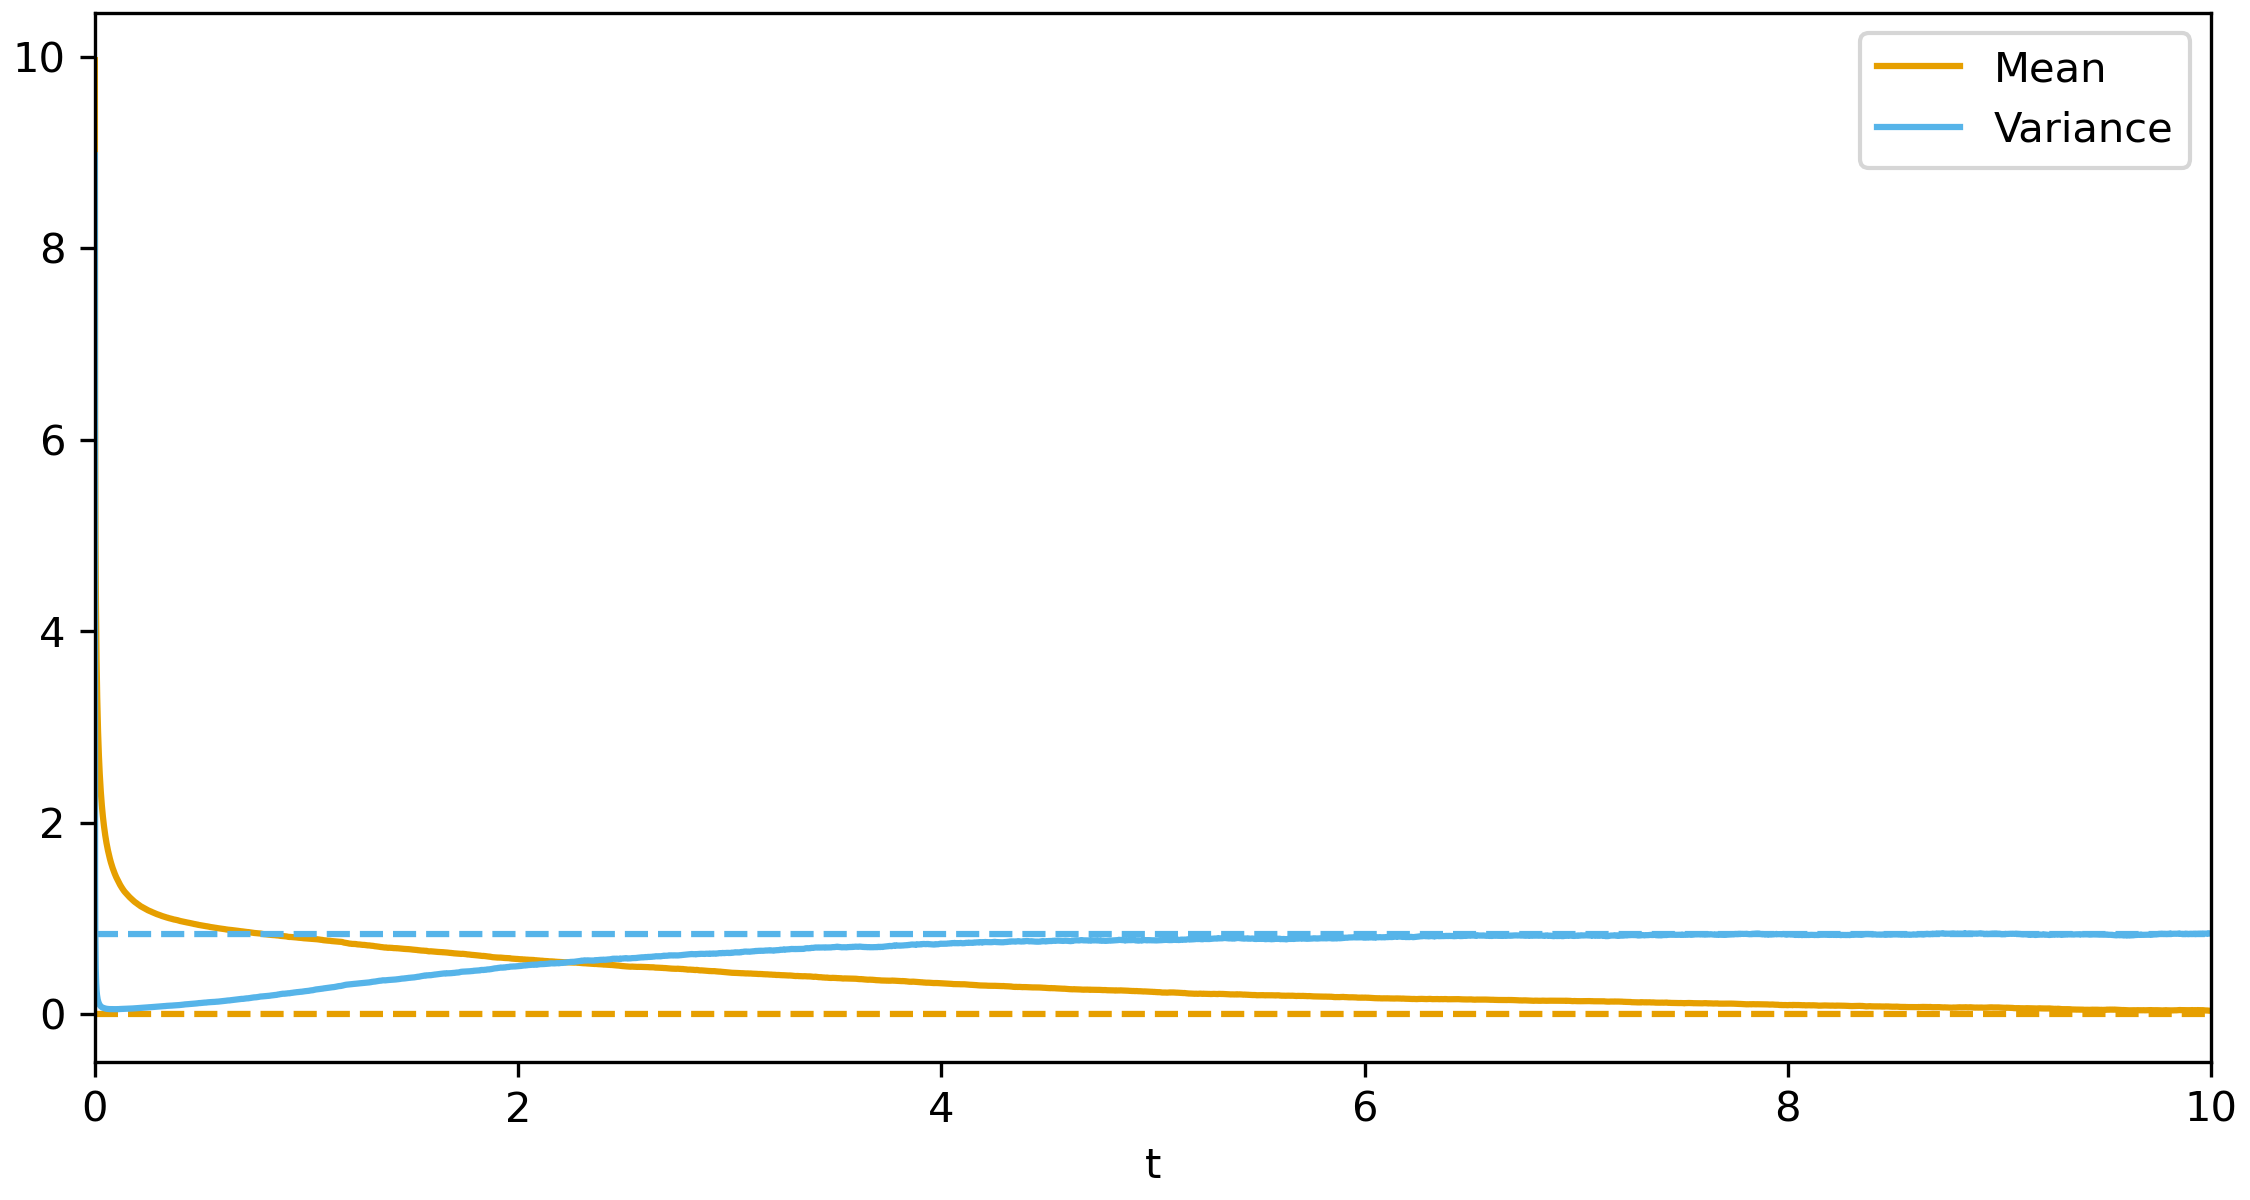
\includegraphics[width=0.75\textwidth]{../../src/6c_evo.png}
		\caption{The evolution of the mean (solid blue) and variance (solid orange) of Eqn.~\ref{eqn:model_6} for 10000 trials of 1000 time-steps of size $dt = 0.001$ with parameters $\sigma = 1$, $F = 0$, $a = 3$, $b = 0$, and $c = 3$, initialized as $x \sim \func{\mathcal{N}}{10,\ 9}$. They rapidly decay toward their equilibrium values (dashed, colored similarly).}
		\label{fig:6c_evo}
	\end{figure}
	
	We find this behavior to be unexpected, as the distribution seems to decay to a Dirac distribution centered on one and then ``expands'' towards their expected equilibrium values.
	
\end{enumerate}